\documentclass{article}
\usepackage[utf8]{inputenc}
\usepackage{tikz}

\begin{document}
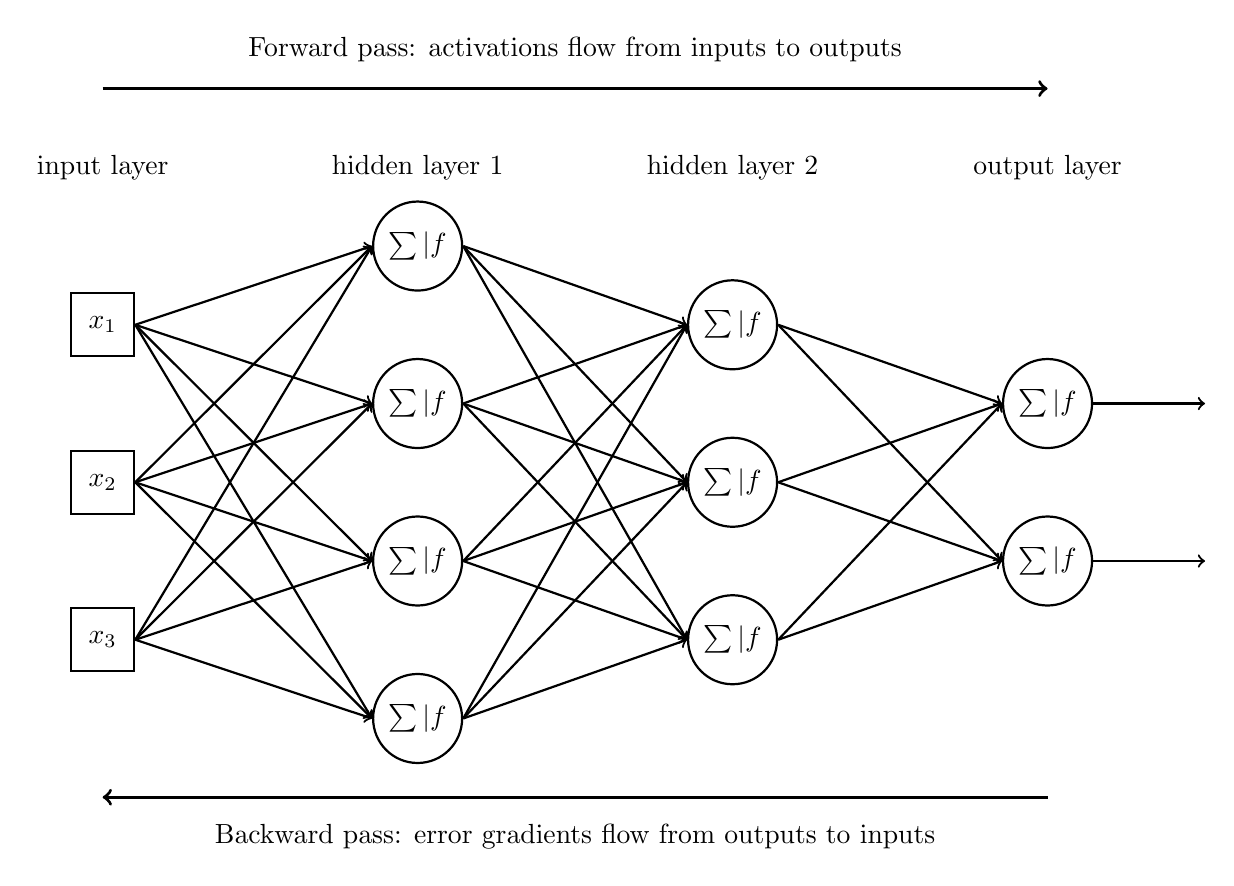
\begin{tikzpicture}
[neuronnode/.style={circle, draw=black, thick, minimum size=10mm},
inputnode/.style={rectangle, draw=black, thick, minimum size=8mm},
connect/.style={->,thick}]
\node at (-4, 4) {input layer};
\node at (0, 4) {hidden layer 1};
\node at (4, 4) {hidden layer 2};
\node at (8, 4) {output layer };
\node[inputnode]	(input1) at (-4, 2) {$x_1$};
\node[inputnode]	(input2) at (-4, 0) {$x_2$};
\node[inputnode]	(input3) at (-4, -2) {$x_3$};
\node[neuronnode]	(neuron1) at (0, 3) {$\sum|f$};
\node[neuronnode]	(neuron2) at (0, 1) {$\sum|f$};
\node[neuronnode]	(neuron3) at (0, -1) {$\sum|f$};
\node[neuronnode]	(neuron4) at (0, -3) {$\sum|f$};
\node[neuronnode]	(neuron5) at (4, 2) {$\sum|f$};
\node[neuronnode]	(neuron6) at (4, 0) {$\sum|f$};
\node[neuronnode]	(neuron7) at (4, -2) {$\sum|f$};
\node[neuronnode]	(output1) at (8, 1) {$\sum|f$};
\node[neuronnode]	(output2) at (8, -1) {$\sum|f$};
\draw[connect] (input1.east) -- (neuron1.west);
\draw[connect] (input1.east) -- (neuron2.west);
\draw[connect] (input1.east) -- (neuron3.west);
\draw[connect] (input1.east) -- (neuron4.west);
\draw[connect] (input2.east) -- (neuron1.west);
\draw[connect] (input2.east) -- (neuron2.west);
\draw[connect] (input2.east) -- (neuron3.west);
\draw[connect] (input2.east) -- (neuron4.west);
\draw[connect] (input3.east) -- (neuron1.west);
\draw[connect] (input3.east) -- (neuron2.west);
\draw[connect] (input3.east) -- (neuron3.west);
\draw[connect] (input3.east) -- (neuron4.west);
\draw[connect] (neuron1.east) -- (neuron5.west);
\draw[connect] (neuron1.east) -- (neuron6.west);
\draw[connect] (neuron1.east) -- (neuron7.west);
\draw[connect] (neuron2.east) -- (neuron5.west);
\draw[connect] (neuron2.east) -- (neuron6.west);
\draw[connect] (neuron2.east) -- (neuron7.west);
\draw[connect] (neuron3.east) -- (neuron5.west);
\draw[connect] (neuron3.east) -- (neuron6.west);
\draw[connect] (neuron3.east) -- (neuron7.west);
\draw[connect] (neuron4.east) -- (neuron5.west);
\draw[connect] (neuron4.east) -- (neuron6.west);
\draw[connect] (neuron4.east) -- (neuron7.west);
\draw[connect] (neuron5.east) -- (output1.west);
\draw[connect] (neuron5.east) -- (output2.west);
\draw[connect] (neuron6.east) -- (output1.west);
\draw[connect] (neuron6.east) -- (output2.west);
\draw[connect] (neuron7.east) -- (output1.west);
\draw[connect] (neuron7.east) -- (output2.west);
\draw[connect] (output1.east) -- (10,1);
\draw[connect] (output2.east) -- (10,-1);
\draw[->, draw=black, very thick] (-4,5) -- (8,5);
\node at (2,5.5) {Forward pass: activations flow from inputs to outputs};
\draw[<-, draw=black, very thick] (-4,-4) -- (8,-4);
\node at (2, -4.5) {Backward pass: error gradients flow from outputs to inputs};
\end{tikzpicture}
\end{document}